\documentclass[conference]{IEEEtran}
\IEEEoverridecommandlockouts
\usepackage{cite}
\usepackage{amsmath,amssymb}
\usepackage{booktabs}
\usepackage{tabularx}
\PassOptionsToPackage{hyphens}{url}\usepackage{url}
\usepackage{tikz}
\usepackage{pgfplots}
\usepackage{microtype}
\usepackage{balance}
\usepackage[hidelinks]{hyperref}
\pgfplotsset{compat=1.16}
\newif\ifanonymous
\anonymousfalse
\ifanonymous
  \hypersetup{pdftitle={Gaming ISO 20022 Payment Messages: An Adversarial Data-Quality Benchmark for Purpose Codes, Party Fields, and Message Paths},pdfauthor={Anonymous}}
\else
  \hypersetup{pdftitle={Gaming ISO 20022 Payment Messages: An Adversarial Data-Quality Benchmark for Purpose Codes, Party Fields, and Message Paths},pdfauthor={Abhishek Sharma}}
\fi
\begin{document}
\title{Gaming ISO~20022 Payment Messages:\\
An Adversarial Data-Quality Benchmark for\\
Purpose Codes, Party Fields, and Message Paths}
\ifanonymous
\author{\IEEEauthorblockN{Author names withheld for double-blind review}
\IEEEauthorblockA{Affiliations withheld for double-blind review}}
\else
\author{\IEEEauthorblockN{Abhishek Sharma}
\IEEEauthorblockA{\textit{Senior Member, IEEE}\\
Independent Researcher\\
abhishek.sharma@ieee.org}}
\fi
\maketitle
\begin{abstract}
ISO~20022 gives payment controls more structured data, but message creators
still decide where names, addresses, and purpose information appear. We study
\emph{message gaming}: deliberate edits to purpose codes, party fields, or the
message path that lower a modelled alert probability while preserving the
payment's business meaning. Purpose-code gaming is the best-known case; the
benchmark also covers misfielding and message-path changes, eleven
manipulations in all. A seeded generator creates synthetic pain.001 and
pacs.008 records, adds ordinary data-quality defects at a controlled rate, and
labels adversarial edits. The evaluation is synthetic and relative to a
published screening abstraction, not to any institution's controls. Each of
three 200{,}000-record runs contains about 5.0\% gamed messages among
benign, defective, and unevaded illicit ones. We also introduce
screening-evasion lift (SEL), which measures how much a manipulation increases
modelled pass-through. Seven detectors are compared, including two standard
reference methods, with every learned model cross-fitted so that no record is
scored by a model that trained on it. Under two-fold cross-fitting, the supervised gradient-boosted model reaches
AUC 0.883 and recovers 16.8\% of gamed messages at an exact
1\% alert capacity, against a ceiling of 20.2\%. It then falls from
AUC 0.769 to 0.377 on a misfielding family withheld from
training, because that family's signature is benign-only in the training
data. The label-free detectors reach AUC 0.750 to 0.777 but recover
only 3.8\% to 10.1\% at the same capacity, and their
ordering by AUC is the reverse of their ordering by recovery. SEL ranges from 1.33 to
1.79 in the main calibration. Detection difficulty does not follow the
P1/P2/P3 action taxonomy; it follows whether an edit leaves a contradiction
inside the message.
\end{abstract}
\begin{IEEEkeywords}
ISO~20022, payment data quality, purpose codes, sanctions screening,
anti-money laundering, adversarial evaluation, synthetic benchmark
\end{IEEEkeywords}

\section{Introduction}
A payment message is both an instruction and a compliance record. Names,
addresses, amounts, and purpose information may feed sanctions, fraud, and
anti-money-laundering controls. The move to ISO~20022 makes much of that
information easier to parse. In CBPR+, purely unstructured party and agent
addresses cease to be supported from 14 November 2026; town and country must
at least appear in designated fields~\cite{swift2026addr}. CPMI's harmonised
data requirements similarly encourage consistent structured data and
registered codes by end-2027, although CPMI is explicit that the requirements
are guidance rather than a regulatory mandate~\cite{cpmi2026}.

Structure does not remove discretion. A message creator still chooses which
optional fields to populate, which purpose code to declare, how much detail to
place in free text, and sometimes which initiation or routing path is used.
Screening is also selective. Published Swift guidance identifies elements that
normally warrant direct screening and allows other fields to provide context
instead~\cite{swiftgp2021}. Purpose and category-purpose codes may influence
processing or monitoring, yet market-practice guidance notes that these codes
are often misunderstood or placed in the wrong field~\cite{pmpg2024}. An
ordinary data-quality error and a deliberate low-scrutiny choice can therefore
leave similar evidence.

That overlap creates a practical evaluation problem. A detector can look good
by finding malformed records, even though malformed records are mostly benign.
It can also earn a high AUC by learning the edit signatures of one generator,
then fail on a manipulation that was absent from training. The relevant
question is narrower than ``can the model spot unusual data?'' It is whether
deliberate changes remain distinguishable from routine error at an alert
capacity a payment operation could actually use.

The work contributes eleven message-level manipulations with explicit
capability assumptions and costs, and a seeded synthetic benchmark with a
tunable ordinary-error floor, a transparent screening abstraction, and
leave-one-family-out testing. It introduces screening-evasion lift (SEL),
which separates an adversary's gain from the portion removed by a detector.
It compares seven detectors, two of them standard reference methods, under
cross-fitting and exact alert capacities with confidence intervals. The central empirical
result is that the taxonomy explains what the adversary changes, but not what
a detector can see. Detectability follows message-internal contradiction
rather than the P1/P2/P3 family label. The detectors are conventional on
purpose; the benchmark, the operational measurement, and the failure cases are
the contribution. No real payment, customer, or institution-specific alert
data is used.

\section{Background and Related Work}
\subsection{Fields and control boundaries}
The benchmark covers customer credit transfers at two stages: pain.001 at
initiation and pacs.008 between financial institutions. Relevant content
includes \texttt{Purp/Cd}, \texttt{CtgyPurp/Cd}, party names and postal
addresses, \texttt{UltmtDbtr}, and structured or unstructured remittance
information. Purpose describes the underlying reason for a transaction;
category purpose is a higher-level instruction that may affect processing.
Their exact use is corridor- and institution-specific, which is why the paper
does not assign a universal risk meaning to any ISO code.

The address transition is useful context but not the attack itself. A hybrid
address can retain free-text lines while placing town and country in their
designated fields. That improves machine readability, but it does not guarantee
that the most informative identity or location evidence sits in a field read
by every control. Likewise, a valid purpose code can still be implausible for
the creditor's industry or inconsistent with the remittance narrative. The
benchmark treats these as consistency questions, not schema errors.

Selective screening is unavoidable. Reading every string as a party name
would create an unmanageable false-positive burden, while ignoring contextual
fields loses useful evidence. The tested controls therefore represent three
layers: structural validation, consistency checks within one message, and
comparison with a synthetic transaction history. Message-level checks can
catch contradictions, but they cannot recover context that has been removed
or shifted to a different path.

\subsection{Related benchmarks and adversarial framing}
Public AML resources operate at the transaction or graph level. The Elliptic
data set labels Bitcoin transactions~\cite{weber2019}, AMLSim simulates
laundering patterns over account graphs~\cite{suzumura2021}, AMLworld models
realistic transaction networks with laundering labels~\cite{altman2023}, and
SAML-D supplies a labelled synthetic monitoring dataset~\cite{oztas2023}.
The more recent AMLgentex and Tide generators add partial observability,
temporal dynamics, and configurable illicit prevalence~\cite{ostman2025,
beukel2026}. Strategic simulations let laundering agents adapt against a
detector~\cite{wang2025}, and directed-multigraph neural networks have been
built to read these graphs~\cite{egressy2024}. All of these resources study
who pays whom, how much, and when. They do not encode the internal placement
of ISO~20022 fields, so they cannot express a manipulation whose mechanism is
that a name, code, or narrative appears in a different element.
Transaction-purpose classification addresses enrichment of missing or noisy
labels, rather than a label selected strategically~\cite{busson2023}. On the
data-quality side, Hammami \emph{et al.} show how noisy free-text party
addresses in real payment traffic degrade parsing even as ISO~20022 adds
structure, and release an augmented benchmark for it~\cite{hammami2024}; that
is the ordinary-error half of the overlap studied here.

Adversarial machine learning on tabular financial data is the closest
methodological line. Ballet \emph{et al.} formalise imperceptibility for
tabular perturbations~\cite{ballet2019}, and Cartella \emph{et al.} adapt
gradient attacks to imbalanced fraud data~\cite{cartella2021}. Simonetto
\emph{et al.} generate feasible examples under domain constraints, combine
gradient and search attacks that respect them, and benchmark tabular
robustness across finance, healthcare, and security
tasks~\cite{simonetto2022,simonetto2024caa,simonetto2024}. Fok
\emph{et al.} show that gradient-based perturbations transfer to tree
ensembles in credit-card fraud detection~\cite{fok2025}. FraudBench
stress-tests policy-grounded banking agents against an adaptive
social-engineering adversary~\cite{pai2026}; it shares the asymmetric
capability framing but operates on dialogue, not on payment messages. Those attacks move numeric feature values under a
norm or a constraint set. The manipulations studied here are discrete,
semantics-preserving edits to a standardised message, whose cost is
operational rather than geometric, and the optimisation follows the classical
cost-bounded evasion setting~\cite{bruckner2011,biggio2013}. Because ordinary
defects and deliberate edits leave similar traces, the benchmark treats the
defect rate $\eta$ as an explicit parameter rather than a fixed property of
the data. Table~\ref{tab:scope} summarises the scope of these adjacent resources.
Numerical comparison across them would be meaningless because the tasks and
data differ; the comparison that can be made is one of scope. The literature
reviewed here does not provide a benchmark that combines message-level field
operations with a controlled accidental-error floor. This is a scoped
observation, not a claim of exhaustive priority.

\begin{table}[!t]
\caption{Scope of adjacent benchmarks as stated by their authors. AML sets:
Elliptic, AMLSim, AMLworld, SAML-D, AMLgentex, Tide~\cite{weber2019,
suzumura2021,altman2023,oztas2023,ostman2025,beukel2026}. Tabular
robustness: \cite{ballet2019,cartella2021,simonetto2022,simonetto2024caa,
simonetto2024}. FraudBench: \cite{pai2026}.}
\label{tab:scope}
\centering
\scriptsize
\begin{tabularx}{\columnwidth}{@{}Xcccc@{}}
\toprule
Dimension & AML sets & Tab. rob. & FraudBench & Ours \\
\midrule
ISO~20022 message elements & no & no & no & yes \\
Field-placement manipulation & no & no & no & yes \\
Adaptive or strategic adversary & partial & yes & yes & yes \\
Explicit ordinary-error floor & partial & no & no & yes ($\eta$) \\
Attacker capability or constraint model & partial & yes & yes & yes \\
Fixed alert-capacity metric & no & no & no & yes \\
Evasion-lift metric & no & no & no & SEL \\
\bottomrule
\end{tabularx}
\end{table}

\section{Threat Model and Manipulations}
The adversary can construct or amend a payment instruction but does not control
a bank's screening system, sanctions lists, or alert threshold. This covers a
corporate originator, a payment-service provider (PSP), or an insider with
legitimate initiation access. Message-path substitution is a stronger
capability: it applies only to a PSP, bank-side actor, or originator that can
choose among available channels. A typical corporate sender cannot simply
select an interbank message type.

A black-box adversary knows public message guidance and receives only a coarse
accept-or-hold outcome; its admissible set excludes the targeted code
substitutions P2a, P2b, and P2d, which require knowing which codes score
lower, but retains code omission (P2c). A grey-box adversary also knows the
relative ordering of the benchmark's purpose-code weights and may use every
primitive. Neither version observes the exact threshold or a production rule
set. The distinction is methodological: it lets the evaluation ask whether
more knowledge makes the evader harder to catch, without suggesting that any
particular bank exposes those weights.

Let $x$ be an illicit synthetic payment instruction, $m$ an admissible
modification, $c(m)$ its operational cost, and $\pi(x)$ the alert probability
in the published screening abstraction. The evader chooses
\begin{equation}
 m^*=\arg\min_m\{\pi(m(x))+\lambda c(m)\}
 \quad\text{s.t.}\quad V(m(x)),\ |m|\leq k,
 \label{eq:evader}
\end{equation}
where $V$ requires the modified record to pass the benchmark's structural and
business checks and preserve the intended transfer. $V$ holds by construction:
every primitive rewrites placement, codes, or path while leaving the amount,
the parties, and the intended beneficiary unchanged, the primitives of a subset
are applied in the order of Table~\ref{tab:taxonomy}, and no pair is mutually
exclusive. This is a cost-bounded,
test-time evasion problem~\cite{bruckner2011,biggio2013}. It does \emph{not}
imply that every generated XML instance would be accepted or settled by a
production bank.

\begin{table}[!t]
\caption{The eleven benchmark primitives with their operational cost $c(m)$.
Costs are illustrative constants on a common scale; they are published with
the code and are not estimates of any actor's effort.}
\label{tab:taxonomy}
\centering
\scriptsize
\begin{tabularx}{\columnwidth}{@{}lXr@{}}
\toprule
ID & Operation & $c(m)$ \\
\midrule
\multicolumn{3}{@{}l}{\emph{P1 misfielding: where identity or address evidence appears}} \\
P1a & move the ultimate-party name into unstructured remittance text & 0.30 \\
P1b & move town and country into a free-text address line & 0.25 \\
P1c & truncate a screened name to four characters & 0.15 \\
P1d & omit the ultimate debtor & 0.20 \\
\multicolumn{3}{@{}l}{\emph{P2 code choice: declared semantics of an intact container}} \\
P2a & replace the purpose code by the lowest-weight plausible code & 0.05 \\
P2b & replace the category purpose & 0.08 \\
P2c & omit the purpose code & 0.04 \\
P2d & declare a salary purpose over a goods or invoice narrative & 0.10 \\
\multicolumn{3}{@{}l}{\emph{P3 structure: message path or decomposition}} \\
P3a & switch between pain.001 and pacs.008 & 0.45 \\
P3b & multiply the in-file split count by 3 to 7, capped at 200 & 0.35 \\
P3c & insert an intermediary as the ultimate party & 0.55 \\
\bottomrule
\end{tabularx}
\end{table}

Table~\ref{tab:taxonomy} lists the primitives. P1 changes where identity or
address evidence appears. P2 leaves the container intact but changes the
declared semantics. P3 changes the message path or decomposition. These
families describe the adversary's action. Whether they also predict
detectability is treated as an empirical question; the evaluation tests that
expectation rather than building it into the detector.

\section{Benchmark and Method}
\subsection{Synthetic population and edits}
The generator draws each message independently. A creditor belongs to one of
six industries, each with a fixed purpose-code profile over eight purpose
codes (for example, a manufacturing creditor receives GDDS with probability
0.45, SUPP 0.30, TRAD 0.15, SERV 0.05, and OTHR 0.05). A debtor--creditor
corridor is drawn from five country pairs with fixed corridor weights, the
category purpose from five codes, the amount from a log-normal distribution
with log-mean 10.2 and log-standard-deviation 1.4, and the message type from
pain.001 and pacs.008 with equal probability. An ultimate debtor is present
with probability 0.75, and a pair identifier drawn from $n/20$ values links
messages that share a synthetic debtor--creditor relationship, so that a
200,000-record run has about twenty messages per pair. Party names are 4 to
16 random letters. Unstructured remittance text is an invoice reference
followed by zero to six words from a small vocabulary and, with probability
0.3, a second reference, so benign lengths spread over a range instead of
taking a few fixed values. The three words that C4 keys on are not in that
vocabulary, since C4 is defined by them. Pain.001 files may contain
ordinary batches, so that multiple transactions are not a perfect gaming
indicator: 30\% of benign pain.001 files are batched, nine in ten of them
with 2 to 49 transactions and the rest with 50 to 200.

A fraction $\eta$ of records receives one ordinary data-quality defect. The
default mix is 35\% purpose content placed in remittance text, 30\% partial
address destructuring, 20\% absent ultimate party, and 15\% absent category
purpose. These proportions are controlled benchmark choices, not measured
industry rates. Their classes follow the types of field-use problems described
by PMPG~\cite{pmpg2024}.

A fraction $\rho$ is then marked illicit for the screening abstraction. For
each illicit record the evader enumerates every subset of admissible
primitives of size at most $k$, applies the subset, and keeps it if
$\pi(m(x))+\lambda c(m)$ falls below the unmodified $\pi(x)$. A perfectly
rational minimum would concentrate on one cheap edit and leave too few samples
for several primitives, so the implementation samples among the kept subsets
and the no-edit option with probability proportional to
$\exp(-(\text{objective}-\text{minimum})/T)$. Illicit records for which the
no-edit option is drawn form the unevaded control group. Ground truth records
the chosen primitives, the alert probability before and after the edit, and
any accidental defect already present.

\subsection{Screening abstraction and calibration}
The incumbent alert model is transparent rather than institution-specific. A
name leg matches listed names against a stated set of screened elements
(party names, town, and country); address lines and remittance text are not
screened, which is the coverage gap P1 exploits. For an illicit record whose
listed name sits in a screened element, the name leg alerts with probability
$P_{\mathrm{name}}$, reduced to $0.39P_{\mathrm{name}}$ when the name has been
truncated below a fuzzy-match length. A score leg combines purpose, corridor,
amount, and completeness,
\begin{equation}
 s(x)=\frac{w_p+w_c+0.2\min(1,a/250{,}000)+0.10\,u+0.08\,t}
 {\sqrt{n_{\mathrm{splits}}}},
 \label{eq:score}
\end{equation}
where $a$ is the amount, $u$ indicates a missing ultimate debtor, and $t$ a
missing town or country, followed by a logistic threshold,
$p_{\mathrm{score}}=1/(1+e^{-8(s-\tau)})$.
The purpose weight $w_p$ runs from 0.08 (SALA) to 0.45 (TRAD), with 0.32 for
an absent code; the corridor weight $w_c$ runs from 0.05 to 0.40. Splitting a
file dilutes the amount term, which is the mechanism behind P3b. A residual
floor $f$ represents controls outside the evader's reach and applies to
illicit records only. The combined probability is
\begin{equation}
 \pi(x)=1-(1-p_{\mathrm{name}})(1-p_{\mathrm{score}})(1-f).
 \label{eq:screening}
\end{equation}
For benign records only the score leg is active. The weights are illustrative
and published with the code. They are not estimates of any bank's rule set.

Calibration deserves explicit treatment because P1 mainly attacks the name
leg and P2 mainly attacks the score leg. Setting the desired baseline alert
probability $\pi_0$ by adjusting only one leg can make the other family
irrelevant. The benchmark instead divides baseline survival multiplicatively
between the two legs using a stated name-share parameter $\sigma$. With
$S=(1-\pi_0)/(1-f)$, the name leg is set to $P_{\mathrm{name}}=1-S^{\sigma}$
directly. $\tau$ is then solved by bisection so that the mean score-leg
probability over an unevaded illicit probe sample of 4,000 records equals
$1-S^{1-\sigma}$. The main setting uses $\pi_0=0.45$ and $\sigma=0.6$, which
solves to $P_{\mathrm{name}}=0.256$ and $\tau=0.768$; a $3\times3$ grid
varies $\pi_0\in\{0.30,0.45,0.60\}$ and $\sigma\in\{0.4,0.6,0.8\}$.

\subsection{Validation features and XML}
Five constraint groups produce detector features. Table~\ref{tab:constraints}
gives their definitions and separates local checks from those needing context.
C1--C2 represent low-cost validation; C3--C4 look for contradictions within a
message; C5 requires pair history. The purpose-history feature reflects the
type of new-code and historical-pattern mismatch described by the Federal
Reserve~\cite{frb2026}. C5 compares a message's declared purpose with the
purposes declared by the same pair's messages in the other cross-fitting
fold, gamed or not; no gaming label enters any feature, and a message does not
contribute to the history used to score it. Six auxiliary
features complete the eleven-dimensional vector: purpose absent, remittance
length, number of address lines, split count, ultimate debtor absent, and a
creditor name of at most five characters. The supervised detectors use a
separate 25-dimensional raw vector: one-hot purpose, category purpose, and
corridor (each with an ``absent'' slot), log amount, split count, ultimate
debtor absent, town absent, and remittance length. The raw vector deliberately
excludes the evader's own objective terms.

\begin{table}[!t]
\caption{Constraint groups and their feature definitions. $q_{\mathrm{ind}}$
is the creditor industry's profile probability of the declared purpose code
(0 when absent).}
\label{tab:constraints}
\centering
\scriptsize
\begin{tabularx}{\columnwidth}{@{}lXl@{}}
\toprule
ID & Feature & Context \\
\midrule
C1 & 1 if the declared purpose code is not in the code list & field \\
C2 & [TwnNm absent] $+$ [Ctry absent] $+$ [an AdrLine carries a town or country token], each 0 or 1 & message \\
C3 & $(1-q_{\mathrm{ind}})$ $+$ [UltmtDbtr absent] & message \\
C4 & 1 if the purpose is SALA and the remittance text mentions goods, invoice, or shipment & message \\
C5 & share of the pair's other-fold messages that declared a different purpose & history \\
\bottomrule
\end{tabularx}
\end{table}

The field-level records can be serialised as pain.001.001.09 or
pacs.008.001.08. The release checks XML well-formedness and exposes an optional
XSD-validation hook when schemas are supplied. No XSD-validation outcome is
used as experimental evidence, and the paper therefore does not claim that all
emitted instances are production-valid. This distinction also avoids
conflating an XSD pass with channel rules, business validation, or settlement.

\subsection{Detectors, reference methods, and cross-fitting}
$D_0=\mathrm{C1}+\mathbb{1}[\mathrm{C2}>1]$ applies the cheap checks.
$D_1=\mathrm{C1}+0.5\,\mathrm{C2}+\mathrm{C3}+1.5\,\mathrm{C4}$ adds the
fixed consistency rules with hand-set weights. $D_2$ is a histogram
gradient-boosted classifier (150 boosting iterations, other settings at the
scikit-learn defaults) trained on the raw vector with gaming labels. $D_3$ is
an isolation forest with 200 trees fitted to the eleven-dimensional feature
vector of benign training rows~\cite{liu2008}. $D_4$ is the per-run sum
$z(D_1)+z(D_3)$; it has no learned fusion weight and uses no gaming labels.
Two standard reference methods are added so that the benchmark's detectors
can be compared with existing techniques on identical inputs. $D_5$ is a
local outlier factor with 20 neighbours~\cite{breunig2000}, fitted in novelty
mode to the standardised benign feature vector. $D_6$ is an $\ell_2$
logistic regression on the standardised raw vector with gaming labels. No
class weighting is used, and no hyperparameter is tuned on the benchmark, so
no validation split is needed. Only $D_2$ and $D_6$ train on gaming labels.
The label-free detectors $D_3$ and $D_5$ still assume a trusted benign
training stream: they use no positive label, but they do rely on knowing that
their training rows are unmanipulated.

Every learned model is two-fold cross-fitted. Records are split by index
parity into two folds; each model is fitted on one fold, restricted to the
rows it is allowed to see, and scores only the other fold. Every reported
score is therefore out-of-fold, and no record is scored by a model that
trained on it. The same fold split serves two further purposes. A record's C5 history is
built from its pair's messages in the other fold only, and the
standardisation statistics behind $D_4$ are taken from the other fold's
scores. A record therefore contributes neither to the history nor to the
normalisation used to score it. $D_0$ and $D_1$ need no fitting. The held-out-family
experiment uses the same split, with the training fold additionally excluding
every record touching the withheld family.

\subsection{Evasion metrics}
AUC measures ranking but not the value of an attack. Let $\pi_0$ be the alert
probability before manipulation and $\pi_m$ after it. We define
\begin{equation}
 \mathrm{SEL}(m)=\frac{1-\pi_m}{1-\pi_0}.
 \label{eq:sel}
\end{equation}
If detector $D$ alerts manipulated and unmanipulated illicit payments at rates
$\delta_m$ and $\delta_0$, the residual lift is
\begin{equation}
 \mathrm{SEL}_{\mathrm{res}}(m,D)=
 \frac{(1-\pi_m)(1-\delta_m)}{(1-\pi_0)(1-\delta_0)}.
 \label{eq:selres}
\end{equation}
SEL of 1 means that the edit provides no modelled benefit. The gap between
SEL and residual SEL is the portion removed by the detector.

\subsection{Evaluation protocol}
The main setting uses $n=200{,}000$ records per seed, seeds 7--9, $\eta=0.15$,
$\rho=0.05$, $k=2$, $\lambda=0.18$, $T=0.10$, $f=0.10$, target $\pi_0=0.45$,
and $\sigma=0.6$. The positive class is the set of gamed records. About
99.4\% of illicit records select at least one edit, so gamed
records make up 5.0\% of each run (9{,}795--10{,}050 per seed). The
negative class is everything else: benign records with or without an
accidental defect, and the 53--61 unevaded illicit records per
seed. We report AUC with a DeLong 95\% interval, average precision (the area
under the precision--recall curve), and the true-positive rate (recovery) at
exact alert capacities of 1\% and 0.1\%, each with a 95\% record-bootstrap
interval from 200 resamples in which the threshold is re-solved. Precision at
1\% capacity is recovery divided by the capacity ceiling, since the number
of alerts is fixed. Because prevalence is about 5\%, no detector can recover more than
capacity divided by prevalence: 20.2\% of gamed records at 1\%
capacity and 2.0\% at 0.1\%. We state these ceilings beside the
results.

Discrete detector scores create ties. A plain ``score above quantile'' rule can
therefore alert far more records than the stated capacity. The implementation
selects every score above the boundary and assigns the tied block the
label-blind fraction needed to fill the capacity exactly. At 1\% of 200,000
records this is 2,000 expected alerts, not all records tied with the 2,000th.
Reported recovery is the expectation under uniform tie-breaking.

For generalisation, the supervised detectors are retrained while one
primitive family is withheld. The evaluation uses $k=1$ and pure-family
messages, preventing a held-out family from leaking through a second
primitive. Each held-out AUC is compared with an in-distribution AUC on the
same rows from a model trained on every family; label-free detectors have no
gap by construction and are shown once. Before the final rerun, the analysis
plan recorded two directional expectations: P1 and P3 would behave similarly
as coverage changes, while P2 would be harder for fixed rules. A family AUC
near chance or SEL near 1 counted against that framing. This was a documented
analysis plan, not an external preregistration. The protocol also varies
$\eta$, $k$, adversary knowledge, and the calibration grid, each on 100,000
records at seed 7. Configuration, seeds, the commit of the harness, and raw
JSON outputs are retained with the release; the numbers reported here were
produced at commit \texttt{378369dbe6e0}.

\section{Results}
\begin{table}[!t]
\caption{Detection results. Panel (a) is the mean $\pm$ standard deviation
over three 200{,}000-record runs; recovery (Rec.) uses exact capacity with
label-blind tie-breaking, precision (Prec.) is recovery divided by the
ceiling, and the last row is the ceiling imposed by capacity and prevalence.
Panel (b) is the mean of three pure-family runs at $k=1$; $n$ is rounded, and
only $D_2$ and $D_6$ are retrained. $^\dagger$trains on gaming labels.}
\label{tab:results}
\centering
\scriptsize
\textit{(a) Main setting}\\[-2pt]
\setlength{\tabcolsep}{2.4pt}
\begin{tabular}{@{}lccccc@{}}
\toprule
Detector & AUC & AP & Rec.@1\% & Prec.@1\% & Rec.@0.1\% \\
\midrule
$D_0$ C1--C2 checks & 0.497$\pm$0.001 & 0.049 & 0.009$\pm$0.000 & 0.043 & 0.001 \\
$D_1$ fixed rules & 0.750$\pm$0.004 & 0.271 & 0.101$\pm$0.003 & 0.500 & 0.020 \\
$D_3$ isolation forest & 0.699$\pm$0.007 & 0.097 & 0.032$\pm$0.003 & 0.160 & 0.005 \\
$D_4$ $z(D_1)+z(D_3)$ & 0.762$\pm$0.005 & 0.168 & 0.055$\pm$0.003 & 0.271 & 0.011 \\
$D_5$ LOF & 0.777$\pm$0.002 & 0.244 & 0.038$\pm$0.004 & 0.189 & 0.014 \\
$D_2$ gradient boosting$^\dagger$ & 0.883$\pm$0.002 & 0.499 & 0.168$\pm$0.001 & 0.832 & 0.020 \\
$D_6$ logistic regression$^\dagger$ & 0.784$\pm$0.004 & 0.313 & 0.127$\pm$0.001 & 0.628 & 0.018 \\
\midrule
Capacity ceiling & -- & -- & 0.202 & 1.000 & 0.020 \\
\bottomrule
\end{tabular}

\vspace{3pt}
\textit{(b) Leave-one-family-out}\\[-2pt]
\setlength{\tabcolsep}{3pt}
\begin{tabular}{@{}lcccccc@{}}
\toprule
Family & $n$ & $D_1$ & $D_4$ & $D_5$ & $D_2$ in $\rightarrow$ out & $D_6$ in $\rightarrow$ out \\
\midrule
P1 misfielding & 3970 & 0.736 & 0.781 & 0.566 & 0.769 $\rightarrow$ \textbf{0.377} & 0.751 $\rightarrow$ 0.368 \\
P2 code choice & 1777 & 0.848 & 0.762 & 0.823 & 0.958 $\rightarrow$ 0.617 & 0.950 $\rightarrow$ 0.668 \\
P3 structure & 3872 & 0.448 & 0.460 & 0.594 & 0.627 $\rightarrow$ 0.473 & 0.466 $\rightarrow$ 0.460 \\
\bottomrule
\end{tabular}
\end{table}

\subsection{Ranking versus recovery at capacity}
Table~\ref{tab:results}(a) separates ranking from useful recovery. At 1\%
capacity, 2,000 alerts must cover about 9{,}910 gamed records, so no
detector can recover more than 20.2\%. Among the label-free
detectors the ordering by AUC ($D_5>D_4>D_1$) is the reverse of the ordering
by recovery. $D_5$ has the best AUC (0.777) and recovers
3.8\%; the fixed rules $D_1$ have the lowest AUC of the three
(0.750) and recover 10.1\%, half of the ceiling, and at 0.1\%
capacity they fill all 200 alerts with gamed records. The precision column
shows the difference: half of $D_1$'s alerts at 1\% are gamed records,
against 27\% for $D_4$ and 19\% for $D_5$. A score
that is high only when a message contradicts itself places those records
ahead of everything else, while the density and forest scores also rank rare
benign combinations highly. Average precision, which weights the top of the
ranking, puts $D_1$ first among the label-free detectors as recovery does;
AUC puts it last. The supervised $D_2$ reaches AUC 0.883 and recovers
16.8\% (83\% of the ceiling, precision
0.832), but it assumes labels that are unlikely to exist for new
manipulations. Three-seed standard deviations are at most 0.007 for
AUC and 0.004 for recovery, and the widest DeLong half-interval is
0.006, so each difference discussed here exceeds its uncertainty.

\subsection{Comparison with reference methods}\label{sec:refmethods}
The two reference methods bracket the benchmark's own detectors. The local
outlier factor $D_5$, given the same eleven features as $D_3$, beats the
isolation forest on every metric (AUC 0.777 against 0.699) and
edges the rule-and-forest combination $D_4$ on AUC, yet recovers less at
1\% capacity. Logistic regression $D_6$ on the same raw features as $D_2$
reaches AUC 0.784 and recovers 12.7\%, 2.6
points above the best label-free detector; the boosted model adds a further
4.1 points. Labels help, and at this capacity the nonlinear
model is worth as much again. Neither reference method changes the
qualitative picture: label-free detection recovers a minority of the
capacity ceiling, and supervised detection recovers most of it only
in-distribution.

Because the generator writes the features the detectors read, we audited
whether any detector's alerts rest on values that benign synthetic traffic
does not produce. In the main setting 1.1\% of gamed records
carry a remittance length or split count outside the benign range, no benign
record does, and at most 5\% of any detector's alert mass
at 1\% capacity falls on such records (seed 7). An earlier generator version
emitted benign remittance text of exactly two lengths; every primitive that
appended text then left a length absent from benign traffic, and a one-line
out-of-range rule recovered the entire 1\% capacity with no false alert. The
audit is kept in the release as a regression check, and the numbers reported
here are from the corrected generator.

\subsection{Generalisation to an unseen family}
Table~\ref{tab:results}(b) shows how brittle the supervised advantage is.
With P1 withheld, $D_2$ falls from 0.769 to 0.377 on the same
rows (per-seed 0.370--0.382), and $D_6$ falls from 0.751 to
0.368. The P2 drop is smaller but still material (0.958 to
0.617). P3 is not separated by any message-level detector: $D_1$
scores 0.448, $D_4$ 0.460, and the withheld $D_2$ 0.473. This
does not prove that P3 is inherently hidden; it shows that the current fields
offer little ranking signal.

A held-out AUC well below 0.5 is a systematic inversion, not an absence of
signal, and its mechanism can be read off the training data. With P1
withheld, an absent ultimate debtor is more common among benign training
records (27\%, the generation rate plus the
accidental-omission defect) than among the remaining gamed ones. The gamed
rate given an absent ultimate debtor is 2.0\%, against
3.2\% when it is present (seed 7, 100{,}000 records,
$k=1$). The model learns absence as evidence of benignity. P1a and P1d both
remove the ultimate debtor, and their held-out AUC against benign traffic is
0.313 and 0.296; P1c, which truncates a name and leaves
the ultimate debtor in place 81\% of the time, scores
0.570. The ordinary-error floor therefore does more than add
noise: it teaches a supervised model that the signature of an unseen
misfielding edit is what routine sloppiness looks like. P1b is rarely
selected on its own (4 pure selections in 100{,}000 records at
$k=1$) because the screening abstraction has no address-based term, so the P1
rows are carried by P1a, P1c, and P1d.

\subsection{Noise floor}
\begin{figure}[!t]
\centering
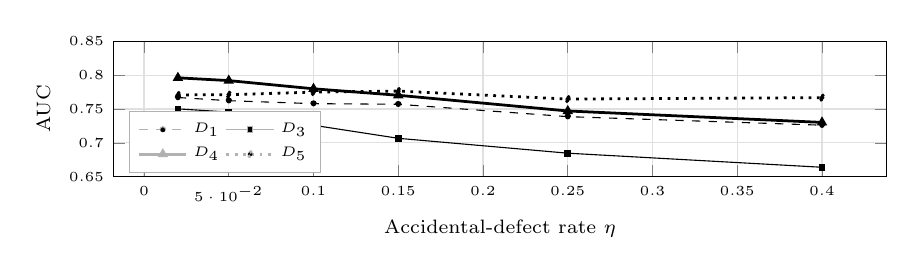
\begin{tikzpicture}
\begin{axis}[
  width=0.94\columnwidth,height=3.3cm,
  xlabel={Accidental-defect rate $\eta$},ylabel={AUC},
  ymin=0.65,ymax=0.85,grid=both,grid style={black!12},
  legend style={at={(0.02,0.03)},anchor=south west,font=\tiny,draw=black!30,legend columns=2},
  label style={font=\scriptsize},tick label style={font=\tiny}
]
\addplot[dashed,mark=*,mark size=1pt] coordinates {(0.02,0.7670) (0.05,0.7623) (0.10,0.7579) (0.15,0.7570) (0.25,0.7387) (0.40,0.7261)};
\addlegendentry{$D_1$}
\addplot[solid,mark=square*,mark size=1pt] coordinates {(0.02,0.7502) (0.05,0.7455) (0.10,0.7260) (0.15,0.7067) (0.25,0.6847) (0.40,0.6639)};
\addlegendentry{$D_3$}
\addplot[solid,line width=1.0pt,mark=triangle*,mark size=1.2pt] coordinates {(0.02,0.7961) (0.05,0.7920) (0.10,0.7799) (0.15,0.7703) (0.25,0.7471) (0.40,0.7302)};
\addlegendentry{$D_4$}
\addplot[dotted,line width=1.0pt,mark=diamond*,mark size=1.2pt] coordinates {(0.02,0.7708) (0.05,0.7712) (0.10,0.7750) (0.15,0.7765) (0.25,0.7647) (0.40,0.7668)};
\addlegendentry{$D_5$}
\end{axis}
\end{tikzpicture}
\caption{AUC as the ordinary defect rate rises. Each point uses 100,000
records at seed 7; only AUC, which is unaffected by threshold ties, is shown.}
\label{fig:eta}
\end{figure}
Fig.~\ref{fig:eta} shows gradual degradation rather than collapse. Raising
$\eta$ from 0.02 to 0.40 lowers $D_4$ AUC by 0.066 and
$D_3$ by 0.086; the fixed rules lose 0.041 and are the
most stable of the benchmark's detectors. The anomaly model degrades fastest
because the benign distribution it learns is itself moving. $D_5$ moves by
no more than 0.012 across the sweep; it keys on rare
combinations rather than on how common the ordinary defects are. At the
highest noise rate every detector still ranks above chance, but the main
operational result warns against treating that ranking as sufficient.

\subsection{Screening-evasion lift}
\begin{figure}[!t]
\centering
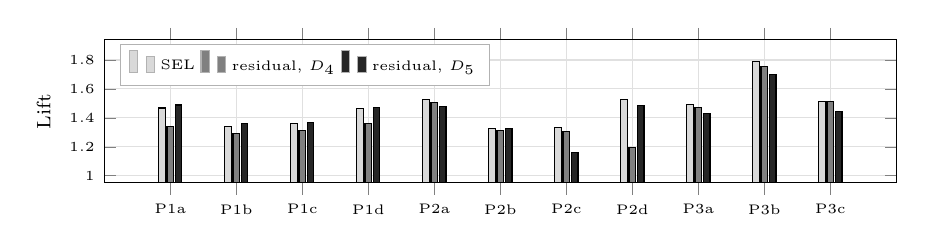
\begin{tikzpicture}
\begin{axis}[
  width=0.96\columnwidth,height=3.4cm,
  ybar=0.6pt,bar width=2.4pt,ylabel={Lift},
  symbolic x coords={P1a,P1b,P1c,P1d,P2a,P2b,P2c,P2d,P3a,P3b,P3c},
  xtick=data,ymin=0.95,ymax=1.94,grid=both,grid style={black!12},
  legend style={at={(0.02,0.97)},anchor=north west,font=\tiny,draw=black!30,legend columns=3},
  label style={font=\scriptsize},tick label style={font=\tiny}
]
\addplot[fill=black!15] coordinates {(P1a,1.468) (P1b,1.339) (P1c,1.361) (P1d,1.466) (P2a,1.528) (P2b,1.327) (P2c,1.334) (P2d,1.524) (P3a,1.495) (P3b,1.792) (P3c,1.514)};
\addlegendentry{SEL}
\addplot[fill=black!50] coordinates {(P1a,1.340) (P1b,1.290) (P1c,1.314) (P1d,1.359) (P2a,1.506) (P2b,1.313) (P2c,1.307) (P2d,1.196) (P3a,1.471) (P3b,1.757) (P3c,1.516)};
\addlegendentry{residual, $D_4$}
\addplot[fill=black!85] coordinates {(P1a,1.489) (P1b,1.363) (P1c,1.370) (P1d,1.469) (P2a,1.478) (P2b,1.325) (P2c,1.161) (P2d,1.486) (P3a,1.433) (P3b,1.701) (P3c,1.446)};
\addlegendentry{residual, $D_5$}
\end{axis}
\end{tikzpicture}
\caption{Mean screening-evasion lift before and after detection at the 1\%
capacity, three seeds. Values are relative to the published screening
abstraction.}
\label{fig:sel}
\end{figure}
Manipulation increases modelled pass-through by
33\%--79\% in the main calibration. Per-seed
95\% bootstrap half-widths from 1,000 resamples are at most 0.025
for SEL and 0.033 for residual SEL, conditional on the observed
unevaded baseline. The detector's value varies sharply by primitive and by
detector. For the code--narrative mismatch P2d, $D_4$ alerts
22.0\% of instances and cuts the lift from 1.524 to
1.196; the residual stays above 1, so the check removes part of the
benefit at this capacity, not all of it. $D_5$ barely touches P2d
(4.2\%) but is the one of the two that reaches the omitted-code
edit P2c (14.5\% against 2.6\%). For in-message
splitting P3b the lift is the largest of all (1.792) and changes little
under either detector (1.757 and 1.701). P3c is starker still
in detection rate: $D_4$ alerts 0.5\% of its instances. At
$k=2$ most gamed messages carry two primitives, so a per-primitive rate
counts a message whichever edit triggered the alert.

Across the three seeds, $D_4$ alerts 0/61, 1/59, 0/53 unevaded illicit
records, so the observed $\delta_0$ is near zero. Replacing each seed's
$\delta_0$ by its exact two-sided 95\% upper bound would raise every
residual value by at most 8\% and changes no
ordering; the small control group remains a reason not to over-interpret
exact values. Across the $3\times3$ calibration grid, SEL ranges from
1.13 to 2.56 while $D_4$ AUC stays between
0.749 and 0.802. The size of the modelled threat is
therefore sensitive to the assumed baseline and name share, while the
relative detection difficulty is more stable. This is why the release reports
the grid rather than treating one SEL number as a deployment estimate.

\subsection{Calibration grid and ablations}
\begin{table}[!t]
\caption{$D_4$ and $D_5$ ablations, 100,000 records at seed 7 per setting.}
\label{tab:ablations}
\centering
\scriptsize
\setlength{\tabcolsep}{3pt}
\begin{tabular}{@{}llcc@{}}
\toprule
Factor & Setting & $D_4$ AUC & $D_5$ AUC \\
\midrule
Family & P1 / P2 / P3 & 0.843 / 0.799 / 0.488 & 0.668 / 0.863 / 0.728 \\
Budget $k$ & 1 / 2 / 3 & 0.649 / 0.770 / 0.844 & 0.614 / 0.776 / 0.845 \\
Knowledge & black / grey & 0.728 / 0.770 & 0.747 / 0.776 \\
\bottomrule
\end{tabular}
\end{table}
Table~\ref{tab:ablations} supports the same interpretation. More edits make
the evader easier to rank: $D_4$ AUC rises from 0.649 at $k=1$ to
0.844 at $k=3$, because each edit can leave another inconsistency.
The grey-box adversary is easier for $D_4$ to detect than the black-box one
(0.770 against 0.728): acting on code-weight knowledge touches
fields that C3--C4 examine. A more informed adversary is therefore not
automatically a stealthier one in this benchmark. Family-only runs put P3 far
below P1 and P2 for $D_4$. For $D_5$ the hardest family is P1
(0.668 against 0.843 for $D_4$), which matches its weak
held-out P1 score in Table~\ref{tab:results}(b); $D_5$ is the stronger of
the two on P2 and P3.

\subsection{What predicted detectability}
The family-level expectations did not survive the rerun. P1 and P3 were both
treated as coverage changes, yet $D_1$ scores 0.736 on P1 and 0.448
on P3. P2, expected to be harder for fixed rules, is $D_1$'s easiest family
at 0.848. The family taxonomy therefore organises the edits but does not
explain the rankings. The sharper distinction is whether an edit leaves a
checkable contradiction. Within P2, $D_4$ alerts 22.0\% of P2d
instances at the 1\% capacity but only
1.6\%--2.6\% of P2a--P2c. Several P1 edits
leave placement or completeness clues, whereas path and decomposition changes
often remain internally coherent. We retain P1/P2/P3 as an action taxonomy,
not a detectability taxonomy.

\section{Discussion and Limitations}
\subsection{Design implications}
The practical lesson is not that structured data weakens controls. It gives
controls better inputs and enables useful consistency checks. The narrower
lesson is that validation, screening coverage, and behavioural monitoring must
be designed together. C1--C2 catch malformed or incomplete data. C3--C4 catch
contradictions within one message. C5 or other longitudinal features are
needed when the message is internally plausible. Changes to path, batch
structure, or party chain may require channel history, agent-chain context, or
comparison with the originator's normal files. A message-only model cannot
infer evidence that the message does not contain. That distinction is the
study's main empirical finding.

The study also separates detector credit from incumbent-control credit. A
primitive can be easy to classify yet offer little extra protection if the
incumbent model would already alert it. Conversely, modest AUC can still be
useful for a narrow primitive if it removes substantial lift at the operating
threshold. SEL and residual SEL make that distinction visible, but they inherit
the assumptions of $\pi$.

\subsection{Limitations}
Several limitations remain. The screening abstraction is transparent and
reproducible, not a reconstruction of a bank's engine, so SEL is a stress
measure rather than an estimate of losses or real evasion. The distributions
of purpose codes, defects, batching, and illicit traffic are assumptions. The
generator and detectors share a feature vocabulary, which can reward
recognition of implementation artefacts; the leave-one-family-out collapse of
the supervised models demonstrates the risk rather than solving it. The
feature vector is discrete, so many records coincide exactly, and
neighbourhood methods such as $D_5$ rank rare combinations rather than smooth
densities; its ranking is therefore sensitive to how the generator populates rare
cells, which the artefact audit of Section~\ref{sec:refmethods} is designed
to expose. Cross-fitting is done within one corpus by index parity, not by
time, so it removes memorisation but does not test drift. External validity
requires recalibration on an institution's own traffic.

The XML layer has a similarly narrow claim. The serializers are checked for
well-formedness, the pain.001 ultimate-debtor ordering was corrected during
review, and the harness accepts external XSDs. The release does not treat XSD
validity as proof of business acceptance. P3a is also capability-dependent and
should not be attributed to an ordinary corporate originator without route
choice. A stronger next experiment would calibrate $\pi$ against anonymised
alert outcomes inside one institution and evaluate path-aware controls without
exporting raw messages.

\subsection{Ethics and responsible release}
The paper enumerates operations that lower a modelled alert probability, so the
release decision deserves a direct answer. None of the eleven operations is
disclosed here for the first time: registered code lists, the harmonised data
requirements~\cite{cpmi2026}, and the published guidance on which elements
normally warrant direct screening~\cite{swiftgp2021} are public, and
market-practice guidance already records purpose codes being placed in the
wrong field~\cite{pmpg2024}. What this work adds is measurement, not
capability. The asymmetry favours the defender: a motivated adversary can
learn which fields an institution reads by observing its own payments, whereas
a control owner has had no structured way to enumerate the coverage gaps that
follow from a selective screening policy. An institution can map the families
onto its own screened fields, message paths, and history features without
disclosing any payment data. The release is deliberately non-operational. The
purpose, corridor, and cost weights are illustrative constants; none is
calibrated against a real corridor, code list, or deployment, and the corpus
contains no customer records, employer data, or production alert outcomes.

\subsection{Artifact availability}
The generator, the evaluation harness, the configuration files, the seeds, and
the raw per-run JSON outputs behind every table and figure are released, with a
notice that the corpora are synthetic and must not be represented as real
payment traffic. Every result file records the commit of the harness that
produced it (\texttt{378369dbe6e0} for the results reported here). A machine-readable summary
collects every number used here, and a verification script re-derives each of
them from the raw outputs. Each number can therefore be reproduced from its
stated seed and configuration, not from a rebuilt approximation. The release
accompanies the submission as supplementary material.

\section{Conclusion}
Some message gaming remains distinguishable from routine error in this
benchmark, and some does not. Edits that leave a contradiction inside the
message, such as a salary code over a goods narrative, are caught by a fixed
consistency rule. Edits that remove or reroute information while leaving the
message coherent, such as path substitution or file splitting, are not
separated by any message-level detector tested here. Good AUC does not imply
useful recovery at a small alert capacity. The label-free detectors reach
AUC 0.750 to 0.777 yet recover 3.8\% to 10.1\%
of gamed messages when 1\% of traffic may be alerted, against a ceiling of
20.2\%, and the best-ranking one recovers the least. A supervised
model closes most of that gap in-distribution and loses it on a family it has
not seen, because the ordinary-error floor makes the unseen family's
signature look benign. The release provides a compact way to test that
boundary and to challenge its assumptions.

\section*{Acknowledgment}
The author used a large language model (Claude, Anthropic) as a research
assistant: to locate and verify prior art, to implement the benchmark
generator, detectors, and evaluation harness, to execute the experimental runs,
and to draft and revise the manuscript. The author defined the research
question and threat model, directed the experimental design, independently
reviewed the code and the raw result files, verified every citation against its
primary source, identified and corrected several methodological defects during
review, and takes full responsibility for all content, claims, and results.

\balance
\begin{thebibliography}{99}
\scriptsize
\setlength{\itemsep}{0pt plus 0.2pt}
\bibitem{swift2026addr}
Swift, ``ISO~20022: The removal of unstructured address,'' Swift Standards,
2026. [Online]. Available:
\url{https://www.swift.com/standards/iso-20022/iso-20022-faqs/iso-20022-removal-unstructured-address}
\bibitem{cpmi2026}
Committee on Payments and Market Infrastructures, \emph{Harmonised ISO~20022
Data Requirements for Enhancing Cross-Border Payments}, Bank for International
Settlements, updated report, Feb. 2026.
\bibitem{swiftgp2021}
Swift, \emph{Guiding Principles for Screening ISO~20022 Payments Messages},
Oct. 2021.
\bibitem{pmpg2024}
Payments Market Practice Group, \emph{ISO~20022 Market Practice Guidance:
Regulatory Reporting, Purpose of Payment and Category Purpose}, ver. 1.1, Jul.
2024.
\bibitem{weber2019}
M. Weber, G. Domeniconi, J. Chen, D. K. I. Weidele, C. Bellei, T. Robinson,
and C. E. Leiserson, ``Anti-money laundering in Bitcoin: Experimenting with
graph convolutional networks for financial forensics,'' in \emph{KDD Workshop
on Anomaly Detection in Finance}, 2019, arXiv:1908.02591.
\bibitem{suzumura2021}
T. Suzumura and H. Kanezashi, ``Anti-money laundering datasets: InPlusLab
anti-money laundering datasets,'' 2021. [Online]. Available:
\url{https://github.com/IBM/AMLSim}
\bibitem{altman2023}
E. Altman \emph{et al.}, ``Realistic synthetic financial transactions for
anti-money laundering models,'' in \emph{Advances in Neural Information
Processing Systems}, vol. 36, 2023.
\bibitem{oztas2023}
B. Oztas \emph{et al.}, ``Enhancing anti-money laundering: Development of a
synthetic transaction monitoring dataset,'' in \emph{Proc. IEEE ICEBE}, 2023,
pp. 47--54.
\bibitem{ostman2025}
J. \"Ostman \emph{et al.}, ``AMLgentex: Mobilizing data-driven research to
combat money laundering,'' arXiv:2506.13989, 2025.
\bibitem{beukel2026}
M. van den Beukel, J. M. Ro\v{z}anec, and A.-L. Varbanescu, ``Tide: A
customisable dataset generator for anti-money laundering research,''
arXiv:2603.01863, 2026.
\bibitem{wang2025}
Q. Wang, W.-T. Tsai, T. Shi, W. Tang, and B. Du, ``Hide and seek in
transaction networks: A multi-agent framework for simulating and detecting
money laundering activities,'' \emph{Complex \& Intelligent Systems}, vol. 11,
art. 271, 2025.
\bibitem{egressy2024}
B. Egressy, L. von Niederh\"ausern, J. Blanu\v{s}a, E. Altman, R. Wattenhofer,
and K. Atasu, ``Provably powerful graph neural networks for directed
multigraphs,'' in \emph{Proc. AAAI Conf. Artificial Intelligence}, vol. 38,
no. 10, 2024, pp. 11838--11846.
\bibitem{busson2023}
A. J. G. Busson \emph{et al.}, ``Hierarchical classification of financial
transactions through context-fusion of transformer-based embeddings and
taxonomy-aware attention layer,'' arXiv:2312.07730, 2023.
\bibitem{ballet2019}
V. Ballet, X. Renard, J. Aigrain, T. Laugel, P. Frossard, and M. Detyniecki,
``Imperceptible adversarial attacks on tabular data,'' arXiv:1911.03274, 2019.
\bibitem{cartella2021}
F. Cartella, O. Anuncia\c{c}\~ao, Y. Funabiki, D. Yamaguchi, T. Akishita, and
O. Elshocht, ``Adversarial attacks for tabular data: Application to fraud
detection and imbalanced data,'' in \emph{Proc. AAAI Workshop on Artificial
Intelligence Safety (SafeAI)}, 2021, arXiv:2101.08030.
\bibitem{simonetto2022}
T. Simonetto, S. Dyrmishi, S. Ghamizi, M. Cordy, and Y. Le Traon, ``A unified
framework for adversarial attack and defense in constrained feature space,''
in \emph{Proc. IJCAI}, 2022, pp. 1313--1319.
\bibitem{simonetto2024caa}
T. Simonetto, S. Ghamizi, and M. Cordy, ``Constrained adaptive attack:
Effective adversarial attack against deep neural networks for tabular data,''
arXiv:2406.00775, 2024.
\bibitem{simonetto2024}
T. Simonetto, S. Ghamizi, and M. Cordy, ``TabularBench: Benchmarking
adversarial robustness for tabular deep learning in real-world use-cases,'' in
\emph{Advances in Neural Information Processing Systems}, vol. 37, Datasets
and Benchmarks Track, 2024.
\bibitem{fok2025}
J. L. Fok, Q. Zeng, S. Chen, O. Fawkes, and H. Chen, ``Foe for fraud:
Transferable adversarial attacks in credit card fraud detection,''
arXiv:2508.14699, 2025.
\bibitem{pai2026}
D. M. Pai and L. Xian, ``FraudBench: Stress-testing policy-grounded banking
agents against adaptive fraud,'' arXiv:2608.18136, 2026.
\bibitem{hammami2024}
H. Hammami, L. Baligand, and B. Petrovski, ``Fighting crime with
Transformers: Empirical analysis of address parsing methods in payment
data,'' in \emph{Proc. NAACL-HLT Industry Track}, 2024, pp. 201--212.
\bibitem{bruckner2011}
M. Br\"uckner and T. Scheffer, ``Stackelberg games for adversarial prediction
problems,'' in \emph{Proc. ACM SIGKDD}, 2011, pp. 547--555.
\bibitem{biggio2013}
B. Biggio \emph{et al.}, ``Evasion attacks against machine learning at test
time,'' in \emph{Proc. ECML PKDD}, 2013, pp. 387--402.
\bibitem{frb2026}
Federal Reserve Financial Services, ``Harnessing the power of ISO~20022: Why
the global payment standard matters for fraud mitigation,'' \emph{Fed360}, 15
Apr. 2026.
\bibitem{liu2008}
F. T. Liu, K. M. Ting, and Z.-H. Zhou, ``Isolation forest,'' in \emph{Proc.
IEEE ICDM}, 2008, pp. 413--422.
\bibitem{breunig2000}
M. M. Breunig, H.-P. Kriegel, R. T. Ng, and J. Sander, ``LOF: Identifying
density-based local outliers,'' in \emph{Proc. ACM SIGMOD}, 2000, pp. 93--104.
\end{thebibliography}
\end{document}
